\renewcommand*{\arraystretch}{1.1}

\subsection*{BI / read / 8}
\label{section:bi-read-08}

\noindent\begin{tabularx}{\queryCardWidth}{|>{\queryPropertyCell}p{\queryPropertyCellWidth}|X|}
	\hline
	query & BI / read / 8 \\ \hline
%
	title & Related topics
 \\ \hline
%
	pattern & \hfill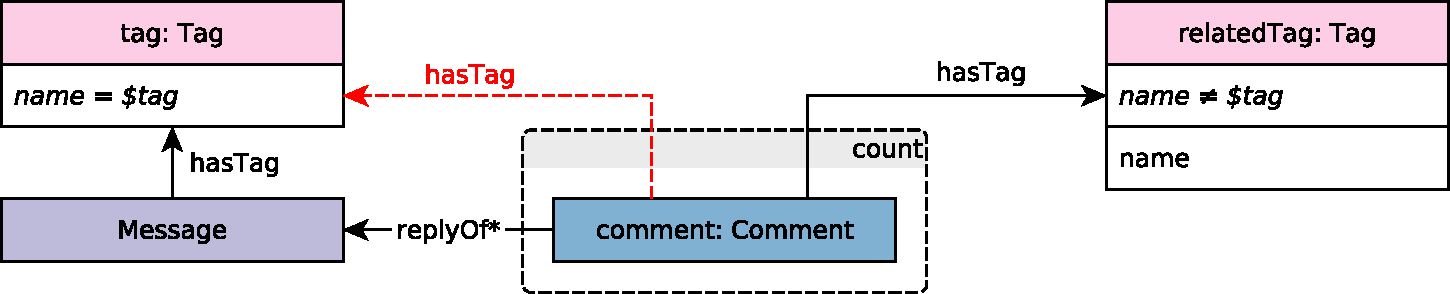
\includegraphics[scale=\patternscale,margin=0cm .2cm]{patterns/bi-read-08}\hfill\vadjust{} \\ \hline
%
	desc. & Find all Messages that have a given Tag. Find the related Tags attached
to replies of these Messages (direct relation not transitive), but only
of those replies that do not have the given Tag.

Group the Tags by name, and get the count of replies in each group.
 \\ \hline
%
	
		params &
		\innerCardVSpace{\begin{tabularx}{\attributeCardWidth}{|>{\paramNumberCell}c|>{\varNameCell}M|>{\typeCell}m{\typeWidth}|Y|} \hline
		$\mathsf{1}$ & tag
 & 32-bit Integer
 &  \\ \hline
		\end{tabularx}}\innerCardVSpace \\ \hline
	
%
	
		result &
		\innerCardVSpace{\begin{tabularx}{\attributeCardWidth}{|>{\resultNumberCell}c|>{\varNameCell}M|>{\typeCell}m{\typeWidth}|>{\resultOriginCell}c|Y|} \hline
		$\mathsf{1}$ & relatedTag.name
 & String
 & R &
				 \\ \hline
		$\mathsf{2}$ & count
 & 32-bit Integer
 & R &
				 \\ \hline
		\end{tabularx}}\innerCardVSpace \\ \hline
	
%
	
		sort		&
		\innerCardVSpace{\begin{tabular}{|>{\sortNumberCell}c|>{\varNameCell}l|>{\directionCell}c|} \hline
		$\mathsf{1}$ & count
 & $\desc
$ \\ \hline
		$\mathsf{2}$ & relatedTag.name
 & $\asc
$ \\ \hline
		\end{tabular}}\innerCardVSpace \\ \hline
	%
	limit & 100 \\ \hline
	%
	CPs &
	\multicolumn{1}{>{\raggedright}l|}{
		\chokePoint{1.6}, 
		\chokePoint{3.3}, 
		\chokePoint{5.2}
		} \\ \hline
	%
	%
\end{tabularx}
\queryCardVSpace